\documentclass[12pt]{article}
%Also I made it 12pt

\usepackage[fontset=macnew]{ctex}
\usepackage{physics}
\usepackage{tikz}
\usetikzlibrary{3d,calc,patterns}
% \usepackage{tkz-euclide}
\usepackage{amsmath}
\usepackage{upgreek}
\usepackage{amsthm}
\usepackage{amsfonts}
\usepackage{mathrsfs}
% \usepackage{subfigure}
\usepackage{subcaption}
%to add an affiliation line to the the title formatting
\usepackage{authblk}

%Fonts
% \usepackage[no-math]{fontspec} %This allows you to enter (via an IPA kayboard) IPA fonts and other symbols directly into LaTeX. Requires a particular setyp, see below.
\usepackage{libertine} %A font that actually contains many IPA symbols. This is the font you see in the preview to the right.

%to use these fonts, be sure that your typesetting engine is set to "XeLaTeX." In Overleaf, go to the Menu link on the top left (by the Overleaf icon), and under Settings be sure that the Compiler is set to "XeLaTeX." If you accessed this document via the Overleaf Pomona Linguistics template, all of this was already done for you.

%The Pomona Linguistics Paper Template in Overleaf is already set up for this, but you may run into this problem if you start building your own documents.


%%%%%%%%%%%%%%%%%%%%%%%%%%%%%%%%%%%%%%%%%%%%%%%%%%%
%packages for this style of handout-formatting of (sub)section headers 
\usepackage[explicit]{titlesec}
\usepackage{xcolor}

\definecolor{light-gray}{gray}{0.7}
\definecolor{lighter-gray}{gray}{0.85}

\titleformat{\section}
{\normalfont\Large\bfseries}{}{0em}{\colorbox{black}{\parbox{\dimexpr\textwidth-2\fboxsep\relax}{\textcolor{white}{\thesection\quad#1}}}}

\titleformat{\subsection}
{\normalfont\large\bfseries\scshape}{}{0em}{\colorbox{light-gray}{\parbox{\dimexpr\textwidth-2\fboxsep\relax}{\textcolor{black}{\thesubsection\quad#1}}}}

\titleformat{\subsubsection}
{\normalfont\bfseries}{}{0em}{\colorbox{lighter-gray}{\parbox{\dimexpr\textwidth-2\fboxsep\relax}{\textcolor{black}{\thesubsubsection\quad#1}}}}
%%%%%%%%%%%%%%%%%%%%%%%%%%%%%%%%%%%%%%%%%%%%%%%%%%%

%%% This file is the preamble for the Pomona Linguistics LaTeX Paper Template, which is also used for the Quick Reference Guide. If you are brand new to writing with LaTeX, we suggest NOT messing with it, and just writing your paper using the Paper Template. If you are getting more comfortable in LaTeX and want to add packages and commands, this is where you do it (when using this template).

%For stacking text, used here in autosegmental diagrams
\usepackage{stackengine}

%To combine rows in tables
\usepackage{multirow}

%geometry helps manage margins, among other things.
\usepackage[margin=1in]{geometry}

%Gives some extra formatting options, e.g. underlining/strikeout
\usepackage{ulem}

%For putting links into papers, also helps make cross-references in the paper smart references
\usepackage[colorlinks = true,
            linkcolor = blue,
            urlcolor  = blue,
            citecolor = blue,
            anchorcolor = blue]{hyperref} %smarter cross-references, these options turn links blue

%Use package/command below to create a double-spaced document, if you want one. Uncomment BOTH the package and the command (\doublespacing) to create a doublespaced document, or leave them as is to have a single-spaced document.
%\usepackage{setspace}
%\doublespacing 

%paragraph formatting
\usepackage[parfill]{parskip}
\setlength{\parskip}{5pt} %plus 1 minus 1}
\setlength{\parindent}{30pt}
\usepackage{titlesec}

%use for special OT tableaux symbols like bomb and sad face. must be loaded early on because it doesn't play well with some other packages
\usepackage{fourier-orns}

%Basic math symbols 
\usepackage{pifont}
\usepackage{amssymb}

%%%Gives shortcuts for glossing. The use of this package is NOT explained in the Quick Reference Guide, but the documentation is on CTAN for those that are interested. MJKD finds it handy for glossing. (https://ctan.org/pkg/leipzig?lang=en)
\usepackage{leipzig}

%Tables
\usepackage{caption} %For table captions
\usepackage{booktabs} %helps format tables

%For citations and bibliography - as of 9.1.2019 we don't explain citations in this Quick Reference Guide, but Pedro Martin's tutorial does (see links in the Guide).
\usepackage{natbib}

%For OT-style tableaux
\usepackage{ot-tableau}

%highlights text with \hl{text}
\usepackage{color, soul}

%Drawing Syntax Trees
\usepackage[linguistics]{forest}

%This specifies some formatting for the forest trees to make them nicer to look at
\forestset{
  nice nodes/.style={
    for tree={
      inner sep=0pt,
      fit=band,
    },
  },
  default preamble=nice nodes,
}

%% For numbered and glossed examples %%
\usepackage{gb4e}



%Changes the \maketitle command to be smaller and take up less space on a page. 
\makeatletter         
\def\@maketitle{   % custom maketitle 
\noindent {\Large \bfseries \color{black} \@title}  \\ \hrule \noindent \@author \\ \@date  
}

%The code below will draw a circle around a piece of text. This is very useful for drawing attention to a word in a data example. use the command \circled{text} where the argument (`text' here) is what you want to be circled. This is illustrated in the Quick Reference Guide and the Paper Template.

\usepackage{tikz}

\newcommand{\circled}[1]{\begin{tikzpicture}[baseline=(word.base)]
\node[draw, rounded corners, text height=8pt, text depth=2pt, inner sep=2pt, outer sep=0pt, use as bounding box] (word) {#1};
\end{tikzpicture}
}


%%%%%%%%%%%%%%%%%%%%%%%%%%%%%%%%%%%%%%%%%%%%%%%%%%%%%%%%%%%%
%%%%%%%%%%%%%%%%%%%%%%%%%%%%%%%%%%%%%%%%%%%%%%%%%%%%%%%%%%%%

% Useful Ling Shortcuts

\RequirePackage{leipzig}
%\RequirePackage{mathtools} % for \mathrlap

% % % Shortcuts  (borrowed from JZ, I'm still unsure exactly what xspace requires)
\RequirePackage{xspace}
\xspaceaddexceptions{]\}}

%This makes the \emptyset command be a nicer one
\let\oldemptyset\emptyset
\let\emptyset\varnothing
\newcommand{\nothing}{$\emptyset$}

%Not all of these are explained in the Quick Reference Guide, but they are here bc they are relevant to some of our students.
\newcommand{\1}{\rlap{$'$}\xspace}
\newcommand{\0}{\rlap{\textsuperscript{$ˆ{\circ}$}}\xspace}
\newcommand{\Lb}[1]{$\text{[}_{\text{#1}}$ } %A more convenient left bracket
\newcommand{\Rb}[1]{$\text{]}_{\text{#1}}$ } %A more convenient left bracket
\newcommand{\gap}{\underline{\hspace{1.2em}}}
\newcommand{\vP}{\emph{v}P}
\newcommand{\lilv}{\emph{v}}
\newcommand{\Abar}{A$'$-} %A more convenient A-bar notation
\newcommand{\ph}{$\varphi$\xspace} %A more convenient phi
\newcommand{\pro}{\emph{pro}\xspace}
\newcommand{\subs}[1]{\textsubscript{#1}} %A more convenient subscript
%\newcommand{\hd}{$^{\circ}$\xspace} %Symbol for printing head / degree symbol
\newcommand{\spells}{$\Longleftrightarrow$} %spellout arrow for morph spellout rules
% \newcommand{\tr}[1]{\textit{t}\textsubscript{\textit{#1}}} %easy traces with subscript
\newcommand{\supers}[1]{\textsuperscript{#1}}

% Abbreviations for glossing, based on Leipzig
\newleipzig{hab}{hab}{habitual}
\newleipzig{rem}{rem}{remote}
\newleipzig{sm}{sm}{subject marker}
\newleipzig{t}{t}{tense}
\newleipzig{aa}{aa}{anti-agreement}
\newleipzig{pron}{pron}{pronoun}
\newleipzig{rec}{rec}{recent}
\newleipzig{om}{om}{object marker}
%\newleipzig{ipfv}{ipfv}{imperfective}
\newleipzig{asp}{asp}{aspect}
\newleipzig{lk}{lk}{linker}
\newleipzig{pcl}{pcl}{particle}
\newleipzig{stat}{stat}{stative}
\newleipzig{ints}{ints}{intensive}
\newleipzig{ascl}{ascl}{assertive subject clitic}
\newleipzig{nascl}{nascl}{non-assertive subject clitic}
\newleipzig{ta}{ta}{tense and/or aspect}
\newleipzig{assoc}{assoc}{associative marker}
\newleipzig{hon}{hon}{honorific}
%\newleipzig{whprt}{wh}{\wh particle}
\newleipzig{sa}{sa}{subject agreement}
\newleipzig{conj}{conj}{conjunction}
%\newleipzig{loc}{loc}{locative}
\newleipzig{expl}{expl}{expletive}
\newleipzig{rcm}{rcm}{reciprocal marker}
\newleipzig{pers}{pers}{persistive}
%\newleipzig{}{}{} %this is just to copy for when I want to add more

%%%%%%%%%%%%%%%%%%%%%%%%%%%%%%%%%%%%%%%%%%%%%%%%%%%%%%%%%%%%
%%%%%%%%%%%%%%%%%%%%%%%%%%%%%%%%%%%%%%%%%%%%%%%%%%%%%%%%%%%%

%A couple of packages that seemed to prefer being called toward the end of the preamble

%This package provides macros for typesetting SPE-style phonological rules.
\usepackage{phonrule}

%For using Greek letters outside of math mode.
\usepackage{textgreek}


%Random, lets us use the XeLaTeX logo. Not important to the template at all.
\usepackage{metalogo}


%%%%%%%%%%%%
%% This is the end of the PREAMBLE
%%%%%%%%%%%

%MJKD note to future self - this preamble is just the section headers + PomLing formatting, but an ordering paradox between the two files made me combine them and re-order fontspec. *shrug* In future if it needs an update, just take the PomLing formatting file and add in the section headers for handouts.

\newcommand{\rmd}{\mathrm{d}}
\newcommand{\deriv}[2]{\frac{\rmd #1}{\rmd #2}}
\newcommand{\pderiv}[2]{\frac{\partial #1}{\partial #2}}
\newcommand{\dpderiv}[2]{\dfrac{\partial #1}{\partial #2}}
\newcommand{\dderiv}[2]{\dfrac{\rmd #1}{\rmd #2}}

\title{光的干涉}
\author{\href{mailto:lai-wei@whu.edu.cn}{Lai Wei}}
\date{\today}

\begin{document}

\maketitle

\section{光的相干性}

\subsection{光的电磁理论}

根据光的电磁理论,光是一种波长在一定范围内的电磁波。

对于一系列沿\(x\)轴正方向传播的单色平面电磁波,其波函数(波动表达式)可以写为
\begin{equation}
E(x, t)=E_0 \cos \omega\left(t-\frac{x}{u}\right)=E_0 \cos \left(\omega t-\frac{2 \pi}{\lambda} x\right)
\end{equation}
\begin{equation}
H(x, t)=H_0 \cos \omega\left(t-\frac{x}{u}\right)=H_0 \cos \left(\omega t-\frac{2 \pi}{\lambda} x\right)
\end{equation}
式中\(u = \dfrac{1}{\sqrt{\varepsilon \mu}}\)式电磁波在介质中的传播速度。

光的强度就是电磁波的平均能流密度,并用\(I\)表示,即
\begin{equation}
I=\frac{1}{2} u \varepsilon E_0^2
\label{17-3}
\end{equation}
式\ref{17-3}表明,在同一种均匀介质中,光的强度与光波中电场强度的振幅的平方成正比。人们往往将电场强度振幅的平方\(E_0^2\)称为相对光强,通常也简称光强。

人们将光在真空中的传播速度与光在介质中的传播速度之比称为该介质的折射率,用\(n\)表示,即
\begin{equation}
    n = \frac{c}{u} = \sqrt{\varepsilon_r \mu_r}
\end{equation}
式中\(\varepsilon_r\)、\(\mu_r\)分别是介质的相对电容率和相对磁导率。对于各向同性的均匀介质,其折射率是一个常量。

\subsection{相干光的获得方法}

从普通光源的发光机制可知,来自两个独立光源的光是非相干光,而来自同一光源的两个不同部分的光也不是相干光。利用普通光源获得相干光的方法的基本原理是把由光源上同一点发出的光设法分成两部分,然后再使这两部分叠加起来。由于这两部分光实际上来自同一点光源,所以它们满足相干条件,因而是相干光。从普通光源获得相干光的方法有两种。一种称为\emph{分波振面法},就是在一个电光源发出的波阵面上取出两个满足相干条件的两个子光源,典型的例子就是杨氏双缝干涉实验中的两个狭缝。另一种称为分振幅法,就是当光投射到两种透明介质的分界面上时,利用反射和折射将光波分成两部分或若干份,由于这几部分光波都来自同一个波列,所以也满足相干条件,例如薄膜干涉、迈克耳孙干涉仪等九江市利用了这种方法。

\subsection{光波的相干叠加与非相干叠加}

\subsubsection{非相干叠加}

若\(S_1\)、\(S_2\)是两个独立的光源,则它们之间的初相位之差\(\left[\varphi_{20} (t) - \varphi_{10} (t)\right]\)是随时间而变的,\(\cos \Delta \varphi_P\)在\(\left[-1, +1\right]\)之间随机取值,于是在足够长的观测时间\(\tau\)内,\(\cos \Delta \varphi_P\)的时间平均值一定是零,即
\begin{equation}
    \frac{1}{\tau} \int_{0}^{\tau} \cos \Delta \varphi_P \rmd t = 0
\end{equation}
于是P点的光强为
\begin{equation}
    I = I_1 + I_2
\end{equation}
即交叠区域中任一点的总光强都等于各列光波在该点点光强之和,这称为非相干叠加。

\subsubsection{相干叠加}

若\(S_1\)、\(S_2\)是两个相干光源,即它们之间的初相位之差\(\varphi_{20} (t) - \varphi_{10} (t) = \varphi_{20} - \varphi_{10}\)与时间\(t\)无关,则\(\cos \Delta \varphi_P\)在观察时间内也与时间\(t\)无关,即
\begin{equation}
    \frac{1}{\tau} \int_{0}^{\tau} \cos \Delta \varphi_P \rmd t = \cos \Delta \varphi_P
\end{equation}
式中
\begin{equation}
    \Delta \varphi_P = \varphi_{20} - \varphi_{10} - \frac{2 \uppi}{\lambda} (r_2 - r_1)
\end{equation}
由此可得P点的光强为
\begin{equation}
I=I_1+I_2+2 \sqrt{I_1 I_2} \cos \Delta \varphi_P=E_{10}^2+E_{20}^2+2 E_{10} E_{20} \cos \Delta \varphi_P
\end{equation}
上式表明,在叠加区域内有些点光强始终加强,有些点光强始终减弱,即各点光强分布不随时间变化,称为相干叠加。

当\(\Delta \varphi_P = \pm 2k \uppi, k=0,1,2,\cdots\)时
\begin{equation}
E_{P 0}=E_{\max }=E_{10}+E_{20}, \quad I=I_{\max }=\left(E_{10}+E_{20}\right)^2
\end{equation}
这称为两列光波在P点满足干涉加强(或相长干涉)条件,P点为第\(k\)级明条纹中心。

当\(\Delta \varphi_P = \pm (2k-1) \uppi, k=1,2,3,\cdots\)时
\begin{equation}
E_{P 0}=E_{\min }=\left|E_{10}-E_{20}\right|, \quad I=I_{\min }=\left|E_{10}-E_{20}\right|^2
\end{equation}
这称为两列光波在P点满足干涉减弱(或相消干涉)条件,P点为暗条纹中心。

特别是当\(E_{10} = E_{20} = E_{0}\)时,\(I_{\mathrm{max}} = 4 E_0^2 = 4 I_0, I_{\mathrm{min}} = 0\)。

\subsubsection{干涉条纹的对比度}

干涉条纹的对比度\(\eta\)定义为
\begin{equation}
    \eta = \frac{I_{\mathrm{max}} - I_{\mathrm{min}}}{I_{\mathrm{max}} + I_{\mathrm{min}}}
\end{equation}
对比度的取值范围\(0<\eta<1\),其中\(\eta=0\)对应于非相干叠加情形;\(\eta=1\)对应于干涉效果最好、干涉条纹明暗对比度最强的相干叠加情形。因此,要获得清晰的干涉图案,除了两列光波需满足振动方向相同、频率相同、相位差恒定这三个必要的干涉 条件之外,还要满足以下两个补充条件:
\begin{enumerate}
    \item 参与干涉的两列光波的振幅不能相差太大。
    \item 场点P到两光源\(S_1\)、\(S_2\)的距离之差\(r_2 - r_1\)不能太大,不能超过一个光源的最大相干长度\(L_m\)。
\end{enumerate}

\section{分波阵面法产生的光的干涉}

\subsection{杨氏双缝干涉实验}

\begin{figure}[!h]
    \centering
    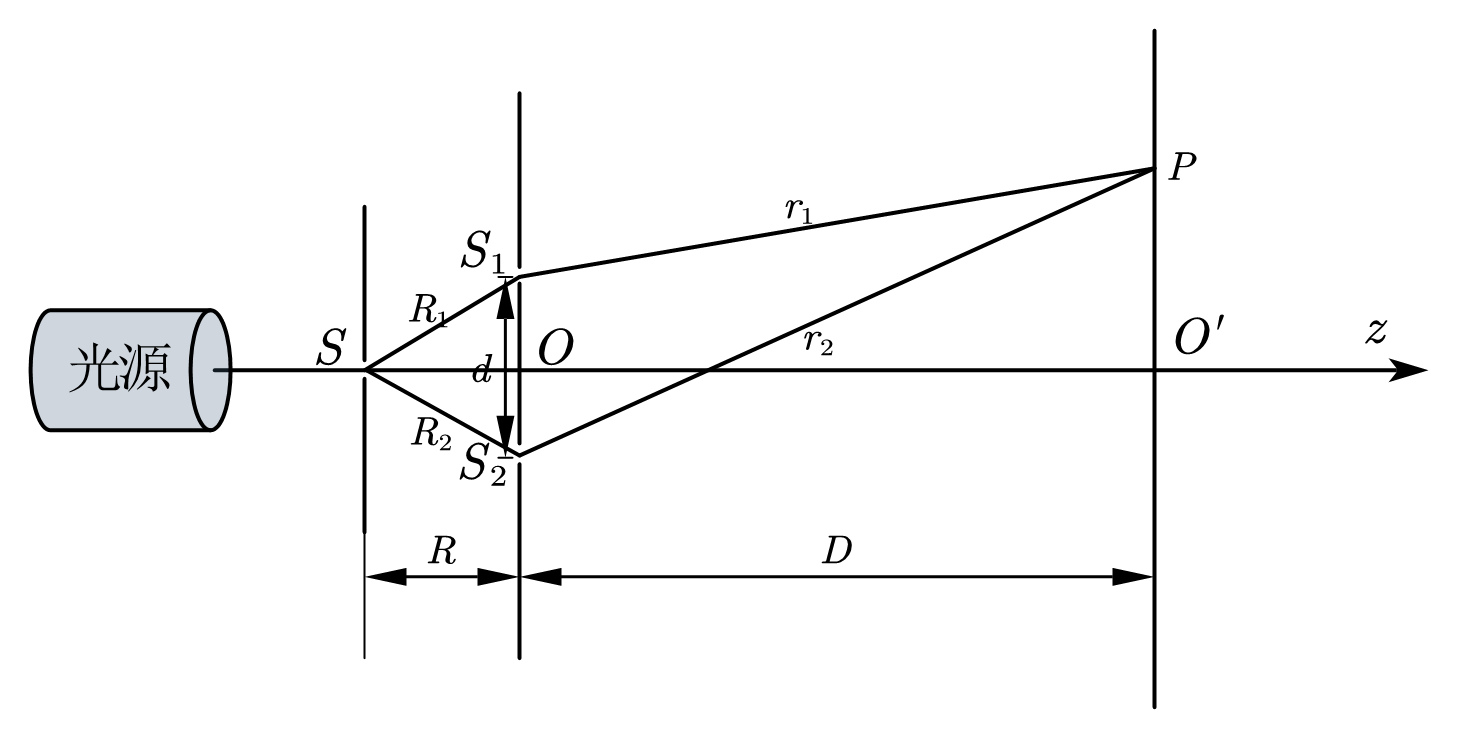
\includegraphics[width=.6\textwidth]{graphics/双缝干涉实验.png}
    \caption{杨氏双缝干涉实验装置示意图}
\end{figure}

设观测屏上任意一点P到坐标原点\(O\)的距离为\(x\),设\(PS_1 = r_1\)、\(PS_2 = r_2\),并假设\(SS_1=SS_2\),则从双缝\(S_1\)、\(S_2\)发出的光波传播到P点时的波程差为
\begin{equation}
    \delta = r_2 - r_1
\end{equation}
由图中几何关系可知
\begin{equation*}
r_1=\sqrt{\left(x-\frac{d}{2}\right)^2+D^2}, \quad r_2=\sqrt{\left(x+\frac{d}{2}\right)^2+D^2}
\end{equation*}
由上面两式可得
\begin{equation}
    r_2^2 - r_1^2 = (r_2 - r_1)(r_2 + r_1) = 2 d x
\end{equation}
在一般的双缝干涉实验中,\(d\)不足1mm,\(D\)通常有几米,故总是可以满足\(D >> d\),所以
\begin{equation}
    r_2 + r_1 \approx 2D
\end{equation}
由此可得
\begin{equation}
\delta=r_2-r_1=\frac{d}{D} x
\end{equation}
可得各级明条纹中心的位置条件为
\begin{equation}
\delta=\frac{d}{D} x= \pm k \lambda
\end{equation}
即
\begin{equation}
x_k= \pm k \frac{D}{d} \lambda \quad(k=0,1,2, \cdots)
\end{equation}
\(k=0\)的明纹常被称为中央明纹或零级明纹。

各级暗条纹中心的位置条件为
\begin{equation}
\delta=\frac{d}{D} x= \pm (2k-1) \frac{\lambda}{2}
\end{equation}
即
\begin{equation}
x_k= \pm (2k-1) \frac{D}{d} \frac{\lambda}{2} \quad(k=1,2,3, \cdots)
\end{equation}
综上,相邻两条明条纹(或暗条纹)之间的距离\(\Delta x\)为
\begin{equation}
\Delta x=x_{k+1}-x_k=\frac{D}{d} \lambda
\end{equation}

\end{document}